% !TeX root = ../proyecto.tex

\chapter{Fundamentos de Aprendizaje Profundo}\label{ch:fundamentos-de-aprendizaje-profundo}
%Fundamentos de Aprendizaje Profundo: Explica los conceptos básicos, incluyendo redes neuronales convolucionales.
\section{Definición de Aprendizaje Profundo}\label{sec:definicion-de-aprendizaje-profundo}
El \textbf{aprendizaje profundo} (Deep Learning)~\cite{weidman_deep_2019} es una subcategoría del aprendizaje
automático que se basa en el uso de \textbf{redes neuronales artificiales} con muchas capas (de ahí el término
``profundo''.
Estas redes están diseñadas para imitar el funcionamiento del cerebro humano, lo que les permite aprender
representaciones complejas de los datos de manera jerárquica. \\[2pt]

La principal diferencia entre el \textbf{aprendizaje automático tradicional} y el aprendizaje profundo es la manera en
que se manejan las características de los datos:
\begin{itemize}
    \item En los enfoques tradicionales, el ingeniero o científico de datos debe extraer manualmente las
          características más importantes para entrenar al modelo (por ejemplo, bordes, formas, texturas en imágenes).
          En el aprendizaje profundo, las redes neuronales son capaces de
          \textbf{aprender automáticamente las representaciones de los datos} a partir de los datos crudos (por ejemplo,
          imágenes, texto, sonido).
    \item Este proceso es denominado \textbf{aprendizaje de características} (feature learning), lo que reduce la
          necesidad de intervención humana.
\end{itemize}

El aprendizaje profundo ha mostrado un rendimiento sobresaliente en diversas tareas, como el reconocimiento de
imágenes, el procesamiento del lenguaje natural, la conducción autónoma y el diagnóstico médico, gracias a su capacidad
para \textbf{capturar patrones complejos} en grandes volúmenes de datos.

\section{Redes Neuronales Artificiales}\label{sec:redes-neuronales-artificiales}
Las \textbf{redes neuronales artificiales} (ANN)~\cite{sydenham_handbook_2005} son el corazón del aprendizaje profundo.
Estas redes están compuestas por neuronas artificiales, que son unidades matemáticas inspiradas en las neuronas
biológicas.
Cada neurona toma varias entradas, las procesa mediante una \textbf{función de activación}, y produce una salida.
Cuando se combinan muchas de estas neuronas en capas, forman una red neuronal.

\subsection{Componentes de una Red Neuronal}\label{subsec:componentes-de-una-red-neuronal}
\begin{enumerate}
    \item \textbf{Neuronas o Unidades}:
          \begin{figure}[htp] \label{fig:neuron}
              \begin{center}
                  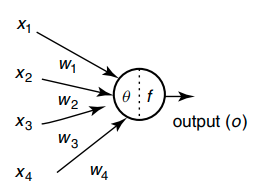
\includegraphics[width=0.5\textwidth]{imagenes/neuron}
              \end{center}
              \caption[Neurona Artificial]{}
          \end{figure}

          Cada \textbf{neurona} realiza una operación simple: recibe varias entradas, las
          pondera por medio de \textbf{pesos} $w_{i}$, suma estos valores junto con un \textbf{sesgo} $b$, y aplica una función
          de activación.
          La salida de la neurona se expresa como:

          $z =w_{1}x_{1} + w_{2}x_{2} + \dots + w_{n}x_{n} + b_{z} = w_{1}x_{1} + w_{2}x_{2} + \dots + w_{n}x_{n} + b$

          Luego, el valor $z$ pasa por una función de activación, que introduce la no linealidad en el sistema, permitiendo que
          las redes neuronales modelen relaciones complejas.
    \item \textbf{Capas de la Red}:
          \begin{figure}[htp] \label{fig:capas-red-neuronal}
              \begin{center}
                  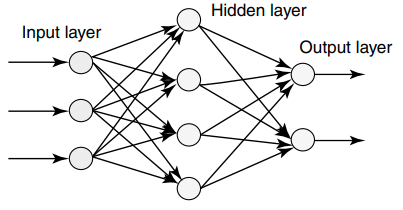
\includegraphics[width=0.5\textwidth]{imagenes/capas_red_neuronal}
              \end{center}
              \caption[Capas de la Red Neuonial Artificial]{}
          \end{figure}
          \begin{itemize}
              \item \textbf{Capa de entrada}: Es la primera capa de la red neuronal, que recibe los datos crudos (por ejemplo,
                    píxeles de una imagen).
              \item \textbf{Capas ocultas}: Estas capas intermedias entre la entrada y la salida aprenden representaciones
                    abstractas de los datos.
                    En una red profunda, hay múltiples capas ocultas, lo que permite la \textbf{transformación jerárquica} de los datos.
              \item \textbf{Capa de salida}: Produce la predicción final, que puede ser una clase (en problemas de clasificación)
                    o un valor numérico (en problemas de regresión).
          \end{itemize}
    \item \textbf{Pesos y Bias}: Los \textbf{pesos} son parámetros ajustables que determinan la importancia de cada
          entrada en la neurona.
          El \textbf{bias} es otro parámetro que se suma al valor ponderado para desplazar la activación de la neurona y permitir
          que el modelo ajuste mejor los datos.

    \item \textbf{Funciones de Activación}: Las funciones de activación son fundamentales para que las redes neuronales
          puedan aprender relaciones no lineales.
          Entre las más comunes se encuentran:
          \begin{itemize}
              \item \textbf{ReLU(Rectified Linear Unit)}: $ReLU(x)=\max(0,x)$, que activa solo valores positivos.
              \item \textbf{Sigmoide}: Que transforma los valores en un rango entre 0 y 1.
              \item \textbf{Tanh (Tangente hiperbólica)}: Transforma los valores en un rango entre -1 y 1.
          \end{itemize}
\end{enumerate}

El uso de \textbf{backpropagation} o retropropagación permite ajustar los pesos y biases durante el entrenamiento
mediante un algoritmo de optimización, como el descenso de gradiente.
De esta manera, la red aprende minimizando la diferencia entre sus predicciones y las respuestas correctas.
\section{Redes Neuronales Convolucionales}\label{sec:redes-neuronales-convolucionales}
Las \textbf{Redes Neuronales Convolucionales} (Convolutional Neural Networks, CNN) son una clase de redes neuronales
profundas especialmente efectivas para el procesamiento de datos que tienen una estructura de tipo rejilla, como las
imágenes.
Fueron inspiradas por el sistema visual de los mamíferos, donde diferentes capas de neuronas responden a estímulos
visuales de manera jerárquica. \\[2pt]

Las CNN son ampliamente utilizadas en tareas de \textbf{visión por computador}, como el reconocimiento de imágenes, la
segmentación de objetos y la clasificación de imágenes.
Lo que diferencia a las CNN de las redes neuronales tradicionales es su capacidad para detectar
\textbf{patrones espaciales} como bordes, texturas, y formas, sin necesidad de un procesamiento manual de las
características.


\subsection{Componentes principales de una CNN}\label{subsec:componentes-principales-de-una-cnn}
\begin{figure}[htp] \label{fig:convolution-layer}
    \begin{center}
        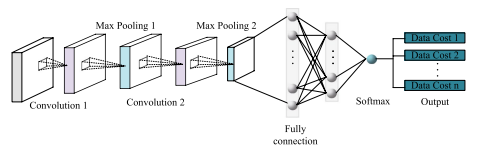
\includegraphics[width=1\textwidth]{imagenes/convolution_layer}
    \end{center}
    \caption[Puntos globales y locales]{En esta imagen extraída de
        \cite{zhao_review_2024} puede observarse de la estructura de una red
        neuronale convolucional. Junto a sus capas convolucionales. }
\end{figure}

\begin{enumerate}
    \item \textbf{Capas Convolucionales}: Estas capas aplican \textbf{filtros o kernels} sobre las imágenes de entrada
          para detectar características locales, como bordes, esquinas o texturas.
          Un filtro convolucional es una pequeña matriz que se mueve a lo largo de la imagen, calculando productos escalares en
          cada posición para producir un mapa de características.

          Las convoluciones son útiles porque explotan la \textbf{localidad de las características}, es decir, las relaciones
          espaciales entre píxeles cercanos.
          Además, la cantidad de parámetros se reduce drásticamente en comparación con las capas densas, ya que el filtro se
          comparte a lo largo de la imagen.
    \item \textbf{Pooling (Submuestreo o Agrupamiento)}: Las capas de pooling reducen la dimensionalidad de las
          características extraídas por las capas convolucionales, lo que hace que las representaciones sean más manejables y
          robustas frente a pequeños cambios o desplazamientos en la imagen.

          El max-pooling es la técnica de pooling más común, donde se toma el valor máximo dentro de una ventana de píxeles,
          reduciendo el tamaño de la imagen, pero reteniendo las características más importantes.
    \item \textbf{Capas Densas}: Después de varias capas convolucionales y de pooling, se agregan una o más
          \textbf{capas densas} (fully connected) para realizar la clasificación o predicción final.
          Estas capas toman todas las características aprendidas en las capas convolucionales y las combinan para generar una
          decisión final.
    \item \textbf{Batch Normalization}: Esta técnica se utiliza para \textbf{normalizar} las salidas de las capas
          intermedias de una red neuronal.
          Batch Normalization ayuda a \textbf{acelerar el entrenamiento} y a hacer que la red sea más estable, al reducir el
          \textbf{desplazamiento covariante} (cambios en las distribuciones de las entradas de las capas intermedias a lo largo
          del entrenamiento).
          Esto se logra al normalizar las entradas de cada capa convolucional o densa antes de aplicar la activación, ajustando
          su media y varianza.

    \item \textbf{Dropout}: El Dropout es una técnica de \textbf{regularización} que se utiliza para prevenir el
          \textbf{sobreajuste} (overfitting) durante el entrenamiento de una red neuronal.
          Durante cada iteración del entrenamiento, Dropout \textbf{desactiva aleatoriamente} un porcentaje de las neuronas, lo
          que obliga a la red a no depender excesivamente de ciertas neuronas y a ser más robusta.
          Esta técnica mejora la generalización de la red, lo que la hace funcionar mejor en datos no vistos.

\end{enumerate}

\subsection{Funcionamiento General de una CNN}\label{subsec:funcionamiento-general-de-una-cnn}
Al pasar una imagen a través de varias capas convolucionales, la red aprende a identificar características simples como
líneas y bordes.
Conforme avanza a capas más profundas, las características se vuelven más abstractas, capturando patrones más complejos
como formas, texturas y, finalmente, estructuras completas como objetos. \\[6pt]

Por ejemplo, en una red entrenada para reconocer caras, las primeras capas pueden detectar bordes o contornos, las
capas intermedias pueden aprender a reconocer ojos, nariz o boca, y las últimas capas pueden identificar una cara
completa.

\subsection{Aplicaciones de las CNN}\label{subsec:aplicaciones-de-las-cnn}
\begin{itemize}
    \item \textbf{Clasificación de imágenes}: Etiquetar imágenes en distintas categorías, como identificar animales o
          vehículos.
    \item \textbf{Detección de objetos}: Identificar y localizar objetos en imágenes.
    \item \textbf{Reconocimiento facial}: Utilizado en sistemas de seguridad, como el desbloqueo de teléfonos móviles.
\end{itemize}

Las CNN son fundamentales en muchas aplicaciones modernas debido a su capacidad para procesar y entender datos visuales
de manera eficiente y automática.

\section{Modelos}\label{sec:modelos}
En el ámbito del aprendizaje profundo, existen diversas arquitecturas de redes neuronales convolucionales que han
demostrado un rendimiento excepcional en diversas tareas de visión por computadora.
Estas arquitecturas están diseñadas para abordar problemas complejos y variados, desde la clasificación de imágenes
hasta la detección de objetos y el segmentado de imágenes. \\[6pt]

A continuación, se explorarán algunas de estas arquitecturas que representan avances significativos en la eficiencia y
efectividad del aprendizaje profundo.

\subsection{ResNet50}\label{subsec:resnet50}
\textbf{ResNet50}~\cite{noauthor_resnet50_nodate} es una arquitectura de red neuronal convolucional introducida por
\texttt{Kaiming He et}~\cite{he_deep_2016}.
La principal innovación de ResNet es la introducción de \textbf{bloques de residualidad}, que permiten la construcción
de redes extremadamente profundas sin el problema de la degradación del rendimiento. \\[6pt]

La idea básica de los bloques residuales es permitir que la red aprenda funciones de identidad, facilitando así la
propagación de la información y el gradiente a través de la red.
En términos prácticos, esto se traduce en un rendimiento mejorado en tareas de clasificación de imágenes, donde
ResNet50 ha logrado resultados sobresalientes en competiciones como ImageNet. \\[6pt]

ResNet50 ha logrado resultados sobresalientes en competiciones como ImageNet~\cite{alnuaim_human-computer_2022}.
Esta arquitectura se compone de 50 capas, de las cuales 49 son convolucionales y una es totalmente conectada,
incluyendo capas de normalización y activación (ReLU), así como conexiones residuales que facilitan el entrenamiento de
redes profundas.

\subsection{MobileNetV2}\label{subsec:mobilenet}

\begin{figure}[htp] \label{fig:resnet50}
    \begin{center}
        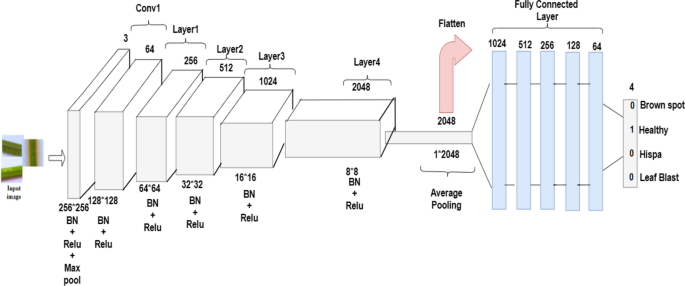
\includegraphics[width=1\textwidth]{imagenes/resnet50}
    \end{center}
    \caption[ResNet50]{Diagrama de la Arquitectuda de ResNet50}
\end{figure}

\textbf{MobileNet}~\cite{howard_mobilenets_2017} es una arquitectura de red neuronal diseñada específicamente para
aplicaciones móviles y de visión por computadora en dispositivos con recursos limitados.
Introducida por Andrew G. Howard et al.\ en 2017, MobileNet se basa en el principio de
\textbf{convoluciones separables en profundidad} (depthwise separable convolutions), que dividen el proceso de
convolución en dos pasos: primero, se aplica una convolución a cada canal de la entrada (depthwise), y luego, se
combinan los resultados con una convolución 1x1 (pointwise). \\[6pt]

Esta técnica reduce significativamente el número de parámetros y el costo computacional, lo que permite ejecutar
modelos de visión por computadora en dispositivos móviles sin sacrificar drásticamente la precisión.

\subsubsection{MobileNetV2}\label{subsubsec:mobilenetv2}

\begin{figure}[htp] \label{fig:mobilenetv2}
    \begin{center}
        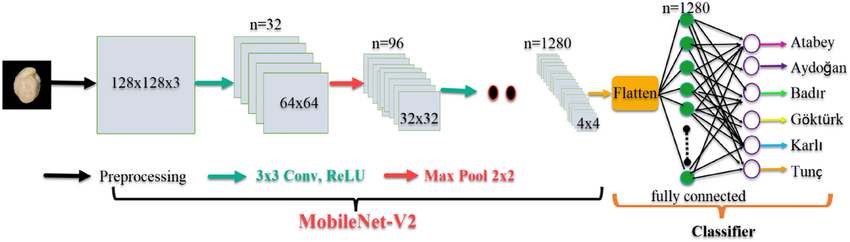
\includegraphics[width=1\textwidth]{imagenes/mobilenetv2}
    \end{center}
    \caption[MobileNetV2]{Diagrama de la Arquitectuda de MobileNetV2}
\end{figure}

\textbf{MobileNetV2}~\cite{sandler_mobilenetv2_2019}, introducido por Sandler et al.\ en 2018, mejora la arquitectura
de MobileNet original al incorporar varias innovaciones.
La principal contribución de MobileNetV2 es la introducción de los bloques de \textbf{residualidad invertida} (inverted
residuals), que permiten que la red mantenga una mayor capacidad de representación y flujo de información a través de
las capas. \\[6pt]

Además, MobileNetV2 utiliza una función de activación llamada \textbf{linear bottleneck}, que ayuda a preservar la
información durante la propagación a través de las capas, lo que mejora aún más el rendimiento del modelo en tareas de
clasificación y detección.
Esta arquitectura se optimiza para ser altamente eficiente, permitiendo que sea utilizada en aplicaciones de tiempo
real en dispositivos con limitaciones de hardware. \\[6pt]

MobileNetV2 ha demostrado ser una opción popular para aplicaciones en dispositivos móviles y sistemas embebidos,
ofreciendo un buen equilibrio entre precisión y eficiencia computacional.
